%!TEX root = main.tex
\Lesson{Функция свёртки}%
\label{Less:fold}

\section[2]{Правая свёртка}%
Важным аспектом программирования является возможность обобщать различные вычислительные процессы, выделяя в~них общую схему вычислений. Мы уже делали это, разрабатывая функцию \s{accumulate,} к~которой сводятся функции \s{sum}, \s{product}, \s{table} и~т.\,д.

Многие функции, обрабатывающие списки имеют одинаковое функциональное <<ядро>>, соответствующее структурной рекурсии, которое можно выделить в форме абстрактной функции обработки списочных структур. 

В качестве примера, рассмотрим определения трёх функций, которые последовательно обрабатывают элементы списка.
Функция \fun{total}{lst} складывает элементы заданного списка; функция \fun{any}{p lst} выясняет, есть ли в списке хотя бы один элемент, удовлетворяющий предикату \lex{p}; и, наконец, функция \fun{map}{f lst} осуществляет отображение списка:
\begin{SchemeCode}[emph={lst,x}]
(define total
  (/. '() --> 0
      (cons h t) --> (+ h (total t))))

(define/c (any p)
  (/. '() --> #f
      (cons h t) --> (or (p h) (any p t))))

(define/c (map f)
  (/. '() --> '()
      (cons h t) --> (cons (f h) (map f t))))
\end{SchemeCode}

Чтобы выделить существенную часть в определениях этих функций, мы использовали форму \s{define/c}, которая позволяет оперировать функциями, как если бы они были каррированы (cм.~стр.~\pageref{define-c}). Таким образом, функция \s{any} имеет два аргумента~--- предикат \lex{p}, заданный в левой части определения, и список~--- аргумент функции\=/подстановки.

Рассмотренные нами три функции имеют очень похожую структуру~--- для некой бинарной функции $f$ и~некоего «нулевого» элемента $x_0$ определяется функция $F$ по~следующей схеме:
\begin{SchemeCode}[emph={lst,x}]
(define F
  (/. '() --> $x_0$
      (cons h t) --> ($f$ h ($F$ t))))
\end{SchemeCode}
\noindent%
Отличаются у этих трёх функций только $f$ и~$x_0$:

\begin{center}
\begin{threeparttable}
\begin{tabular}{>{\schemestyle}llc}\toprule
\multicolumn{1}{c}{$F$} & \multicolumn{1}{c}{$f$} & $x_0$\\\midrule
total & $x, y \rightarrow  x + y$ & \constantstyle 0\\
any & $x, y \rightarrow  (or~(p~x)~y)$ & \constantstyle{\#f}\\
map & $x, y \rightarrow  ((f~x)\ .\ y)$ & \schemestyle '()\\\bottomrule
\end{tabular}
\end{threeparttable}
\end{center}

Выделим функциональное ядро этих функций и~назовём его \index{свёртка!списка! правая}\emph{правой свёрткой}:\label{foldr}

\fnindex{foldr}
\begin{SchemeCode}[emph={f,h,t}]
(:: foldr ((A B -> B) B (list: A ..) -> B)
 (define/c (foldr f $x_0$)
   (/. '() --> $x_0$
       (cons h t) --> (f h (foldr f $x_0$ t))))
\end{SchemeCode}

Обратите внимание на~описание типа функции \s{foldr}. Первым её аргументом должна быть сворачивающая функция двух аргументов, вторым~--- «нулевой» элемент, а~третьим~--- список. При~этом типы элементов списка и~«нулевого» элемента должны соответствовать типам аргументов сворачивающей функции. На~выходе мы получаем результат того же типа, что возвращает сворачивающая функция.

Фактически, эта рекурсивная функция, применённая к~некоему списку, выполняет следующее преобразование:
\begin{SchemeCode}[emph=f]
        (foldr f $x_0$ '(a b c)) $\rightarrow$ (f a (f b (f c $x_0$)))
\end{SchemeCode}
Иными словами, для списка \s{'(a b c)} функция \s{foldr} делает формальную замену: \s[emph=f]{cons $\rightarrow$ f}, \s{null $\rightarrow$ $x_0$}
так, что получается преобразование:
\begin{SchemeCode}[emph=f]
    (cons a (cons b (cons c '()))) $\rightarrow$ (f a (f b (f c $x_0$)))
\end{SchemeCode}

\newpage\noindent
Например, для рассмотренных нами функций:

\begin{SchemeCode}
total:  
 cons $\rightarrow$ +,  '() $\rightarrow$ 0  
 (a . (b . (c . '()))) $\rightarrow$ (a + (b + (c + 0)))%\smallskip%
any: 
 cons $\rightarrow$ (lambda (x y) (or (p x) y)), '() $\rightarrow$ #f  
 (a . (b . (c . '()))) $\rightarrow$ (or (p a) (or (p b) (or (p c) #f)))%\smallskip%
map:
 cons $\rightarrow$ (lambda (x y) (cons (f x) y)), '() $\rightarrow$ '() 
 (a . (b . (c . '()))) $\rightarrow$ ((f a) . ((f b) . ((f c) . '())))
\end{SchemeCode}

Теперь мы можем выразить наши три рекурсивные функции через правую свёртку:

\begin{Definition}[emph={lst,x,y,lst1,lst2,p}]
(define (total lst)
  (foldr + 0 lst))%\medskip%
(define (any p lst)
  (foldr (lambda (x y) (or (p x) y)) #f lst))%\medskip%
(define (map lst1 lst2)
  (foldr (lambda (x y) (cons (f x) y))  lst1)) 
\end{Definition}

С помощью операторов, описанных на стр.~\pageref{operators} и бесточечной нотации (стр.~\pageref{tacit}), удобно давать чисто операторные определения функциям, использующим свёртку:

\label{fold:map}
\begin{Definition}[emph={f,p,test?}]
(define/c (total)  (foldr + 0))%\medskip%
(define/c (any p)  (foldr ($\circ$ or p) #f))%\medskip%
(define/c (map f)  (foldr ($\circ$ cons f) '()))%\medskip%
\end{Definition}

Такие определения не~всегда улучшают читаемость программы, однако они повышают её модульность, что увеличивает надёжность, упрощает отладку программы и~доказательство её корректности.

При~разработке функции, использующей свёртку, полезно мыслить по~следующей схеме: представляем себе исходный список в~виде цепочки вложенных пар: \s{(a . (b . (c . '())))} и~решаем, что мы должны сделать с~каждым элементом списка, на~что мы заменим операцию \s{(.)} и~с чего начинать свёртку. Функция с~помощью которой мы сворачиваем список имеет два аргумента: первый~--- это текущий элемент списка, второй~--- текущий результат свёртки.

Например, мы хотим написать функцию, возвращающую сумму квадратов всех элементов списка. Значит, мы должны сделать преобразование: 
\textrm{\normalfont($a$ . ($b$ . ($c$ . '()))) $\rightarrow$  $a^2$ + ($b^2$ + ($c^2$ + 0))}.  
Сворачивающая функция может выглядеть так:  $f(el,res) = el^2+res$.

\begin{Assignment}
Напишите, используя свёртку, определения следующих функций:

 а) \fun{every}{test? lst} --- возвращает \s{#t} тогда, когда все элементы списка \lex{lst} удовлетворяют предикату \lex{test?}.\vspace{-\smallskipamount}
\begin{Specification}
(test (every odd? '(1 3 5))
      (not (every odd? '(1 2 3))))
\end{Specification}

 б) \fun{count-if}{test? lst} --- подсчитывает число вхождений в список \lex{lst} элементов, удовлетворяющих предикату \lex{test?}.\vspace{-\smallskipamount}
\begin{Specification}
(test (count-if odd? '(1 2 3))  ==> 2
      (count-if odd? '(0 2 4))  ==> 0
      (count-if odd? '())       ==> 0)
\end{Specification}

 в) \fun{count}{el lst} --- подсчитывает число вхождений элемента \lex{el} в~список \lex{lst}. Здесь воспользуйтесь функцией \s{count-if}, написанной вами ранее. \vspace{-\smallskipamount}
\begin{Specification}
(test (count 1 '(2 1 2 1 1))  ==> 3
      (count 3 '(2 1 2 1 1))  ==> 0
      (count 3 '())           ==> 0)
\end{Specification}
\end{Assignment}

\section[2]{Левая свёртка}\index{свёртка!списка!левая}%
Рассмотрим, как может быть реализована функция \si{reverse}, возвращающая список с~элементами, данными в~обратном порядке. Вспомним, что вычисление правой свёртки начинается с~конца списка. Значит, если мы будем сворачивать список функцией \s{appendr}:
\begin{SchemeCode}[emph={x,lst}]
(define (appendr x lst)
  (append lst (list x)))
\end{SchemeCode}

\noindentто каждый следующий элемент будет приклеиваться к~результату справа и~мы получим то, что нужно:

\begin{SchemeCode}
(a . (b . (c . '()))) arrow
arrow (append (append (append '() '(c)) '(b)) '(a)) arrow
arrow (c . (b . (a . '())))
\end{SchemeCode}

Таким образом, получаем определение:

\begin{Definition}
(define (reverse lst)
  (foldr appendr '() lst))
\end{Definition}

Однако эта функция неэффективна: она, проходя по~списку, вынуждена проходить по~каждому вызову \s{append} все достраиваемые подсписки. Таким образом, для списка из~$N$ элементов эта функция совершает $N^2/2$ операций \s{cons}. Вот если бы свёртка осуществлялась не~с конца, а~с начала списка, то можно было бы обойтись использованием только функции \s{cons}. Напишем такую функцию свёртки:

\fnindex{foldl}
\begin{Definition}[emph={f,h,t}]
(:: foldl ((A B -> B) B (list: A ..) -> B)
 (define/c (foldl f $x_0$)
   (/. '() --> $x_0$
       (cons h t) --> (foldl f (f h $x_0$) t))))
\end{Definition}

\noindent
Она выполняет следующее преобразование:

\begin{SchemeCode}
      (foldl $f$ $x_0$ '(a b c))  $\rightarrow$  ($f$ c ($f$ b ($f$ a $x_0$)))
\end{SchemeCode}

\noindent Заметим, что список сворачивается слева направо, поэтому такая свёртка называется \emph{левой}. Обратите так же внимание на~то, что левая свёртка реализует итеративный процесс.

С помощью левой свёртки, функция \s{reverse} выражается очень просто и эффективно:
\begin{SchemeCode}
(define reverse (foldl cons '()))
\end{SchemeCode}

\begin{Assignment}
Определите через свёртку следующие универсальные функции:

\s{(length $lst$)} --- возвращает длину списка $lst$.

\s{(max $lst$)} --- возвращает максимальный элемент списка $lst$.

\fun{filter}{test? lst}~--- фильтрует список \lex{lst}, оставляя в~нём только те элементы, которые удовлетворяют условию \lex{test?}.
\medskip

 \fun{append}{lst1 lst2}~--- объединяет списки \lex{lst1} и \lex{lst2} в один.
\medskip

 \fun{member?}{el lst}~--- отвечает на~вопрос: содержит~ли список \lex{lst} элемент \lex{el}?
\medskip

 \fun{compose}{f \ddd}~--- композиция произвольного числа функций. При этом самая правая функция может принимать сколько угодно аргументов, а прочие~--- унарны.
\medskip

\label{remove-duplicates} \fun{remove-duplicates}{lst}~--- возвращает список уникальных элементов списка \lex{lst}.
\medskip

\fun{from-digits}{digit-list base}~--- возвращает целое число в десятичной системе исчисления, состоящее из~цифр, перечисленных в~списке \lex{digit-list}, используя основание \lex{base}. Если основание не задано, функция должна использовать десятичную систему.
\begin{Specification}
(test 
  (from-digits '(1 2 3))   ==> 123  ;основание 10
  (from-digits '(1 0 0) 2) ==> 4)   ;основание 2
\end{Specification}
\end{Assignment}

\section{Абстракция структурной~рекурсии}%
\index{абстракция!структурной рекурсии}%
Мы увидели, что через свёртку можно выразить множество разнообразных функций, обрабатывающих списки. Такая универсальность не случайна. Вспомним, как определяется абстрактный тип для списков:
\begin{SchemeCode}
(define-type List 
  '()
  (cons: Any List))
\end{SchemeCode}

\noindent
Абстрактные типы, построенные таким образом, называют \index{тип!алгебраический}\emph{алгебраическими}. Они определяются, через \emph{суммы} и \emph{произведения} типов. Сумма типов представляется с помощью объединения, а в качестве операции <<перемножения>> может выступать любая функция\=/констуктор, имеющая более одного агрумента. В случае типа \s{List} --- это сумма единичного типа \s{'()} и произведения типов \s{Any} и \s{List}, выполненного с помощью конструктора \s{cons}.

Определение любой структурно-рекурсивной функции обязательно должно содержать в себе правила для всех слагаемых обрабатываемого алгебраического типа и рекурсивные вызовы. Свёртка является наиболее общей структурно-рекурсивной функцией, описывающей что делать со всеми слагаемыми и множителями в произведениях типов, и вызывающая саму себя для рекурсивных множителей.
Таким образом, она является \emph{абстракцией структурной рекурсии}, и значит, её можно определить для всякого индуктивного множества. 

В качестве примера, построим свёртку для множества натуральных чисел, тип для которых формально можно записать так:
\vspace{-\bigskipamount}
\begin{SchemeCode}
(define-type Nat
  0
  (+ 1 Nat))
\end{SchemeCode}

\noindent
Нам необходимо описать обработку базового случая \s{0} и произведения \s{(+ 1 Nat)}:
\begin{Definition}
(:: nat-fold ((Nat A -> A) A Nat -> A)
  (define/c (nat-fold f x0)
    (/. 0 --> x0
        (+ 1 x) --> (f x (nat-fold f x0 x)))))
\end{Definition}
Посмотрим, как работает эта функция:
\REPLin{(define-formal f g)}
\REPL
  {(fold-nat f 'x0 3))}
  {'(f 3 (f 2 (f 1 x0)))}

Использование свёртки увеличивает модульность программы, гарантирует завершаемость и корректность обработки данных принадлежащих к алгебраическим типам.

\section[2]{Свёртка деревьев}%
\index{свёртка!дерева}
В~самом общем случае, любые заквотированные выражения представляют собой списки списков, то есть, древообразные структуры, или просто \emph{деревья}. Структуру такого дерева можно показать следующим образом: в~узлах находится конструктор \s{cons}, а~листьями являются атомы. На левом рисунке показано дерево, соответствующее выражению \s{'((a (b)) (c d e))}.
\begin{center}\label{fig:tree}
  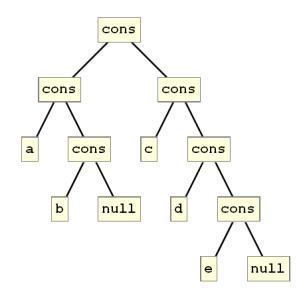
\includegraphics[width=0.41\textwidth]{../figures/tree1.jpg}
  \qquad
  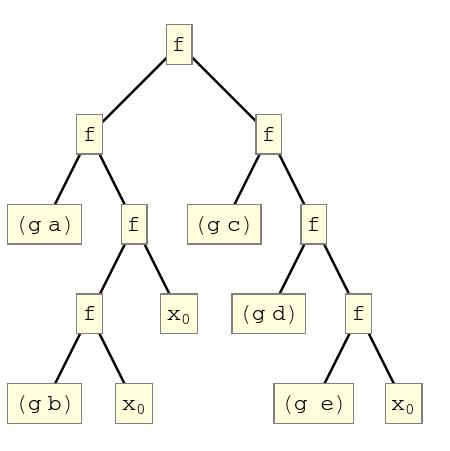
\includegraphics[width=0.41\textwidth]{../figures/tree4.jpg}
\end{center}

Так как \s{cons}~--- бинарная функция, из каждого узла может выходить только две ветви. Такие деревья называются \emph{бинарными}. 

Определим тип для бинарного дерева следующим образом:
\begin{Definition}
(define-type (BTree A)
  '()
  (cons: (BTree A) (BTree A))
  A)
\end{Definition}

Имея выражение для типа, можно сразу дать определение свёртки для него, описав, что делать с каждым слагаемым, и организуя рекурсивные вызовы для рекурсивных множителей в произведении типов:
\fnindex{tree-fold}
\begin{Definition}[emph={f,g,a,l,r}]
(:: tree-fold ((A A -> A) (Any -> A) A (BTree Any) -> A)
 (define/c (tree-fold f g $x_0$)
   (/. '() --> $x_0$
       (cons l r) --> (f (tree-fold f g $x_0$ l) 
                        (tree-fold f g $x_0$ r))
       a --> (g a))))
\end{Definition}
Результат свёртки выражения \s{'((a (b)) (c d e))} показан на правом рисунке на стр.~\pageref{fig:tree}.

Теперь мы можем написать, например, расширения на~случай деревьев для функций \s{length} и~\s{total}: назвав их, соответственно, \si{leaf-count} и~\si{leaf-total}:

\begin{SchemeCode}
(:: leaf-count ((BTree Any) -> Nat)
 (define leaf-count 
   (tree-fold + (const 1) 0)))

(:: leaf-total ((BTree Num) -> Num)
 (define leaf-total 
   (tree-fold + id 0)))
\end{SchemeCode}

Вот --- определение функции \si{flatten}, возвращающей список листьев дерева:
\begin{SchemeCode}
(:: flatten ((BTree Any) -> list?)
 (define flatten 
   (tree-fold append list '())))
\end{SchemeCode}

\newpage
\begin{Assignment}
а) Выразите через свёртку натуральных чисел \s{nat-fold} функцию \s{accumulate} (Задание \ref{accumulate}, стр.~\pageref{accumulate}) и наоборот.

б) Напишите определения следующих универсальных функций для деревьев:

 \fun{leaf-map}{f tree}~--- возвращает дерево \lex{tree}, ко~всем листьям которого применяется функция \lex{f}.
\begin{Specification}
(test 
  (leaf-map sqr '((1 2) (3 (4))))  ==> '((1 4) (9 (16)))
  (leaf-map odd? '(1 (2 (3) 2) 1)) ==> '(#t (#f (#t) #f) #t)
  (leaf-map list '(1 2 3))         ==> '((1) (2) (3))
  (leaf-map list 3)                ==> '(3)
  (leaf-map sqr '(1. 12))          ==> '(1. 144))
\end{Specification}

 \fun{find}{test? tree}~--- возвращает список листьев дерева \lex{tree}, которые удовлетворяют условию \lex{test?}.
\begin{Specification}
(test 
  (find odd? '(1 (2 (3) 2) 1))   ==> '(1 3 1)
  (find odd? '(1 2 3 4))         ==> '(1 3)
  (find zero? '(1 (2 (3) 2) 1))  ==> '())
\end{Specification}

\fun{filter}{test? tree}~--- возвращает дерево с~той же структурой, что и~\lex{tree}, но в~котором присутствуют только листья, удовлетворяющие условию \lex{test?}.
\begin{Specification}
(test 
  (filter odd? '(1 2 3 4))              ==> '(1 3)
  (filter odd? '((1 2) (3 4)))          ==> '((1) (3))
  (filter odd? '(0 (1 (2 (3 4)))))      ==> '((1 ((3))))
  (filter negative? '(0 (1 (2 (3 4))))) ==> '(((())))
  (filter odd? 6)  #f)
\end{Specification}

в) Напишите функцию свёртки для типа <<размеченное дерево>>:
\begin{SchemeCode}
    Tree(A) ::= Empty
             |  Node(A, Tree(A), Tree(A))
\end{SchemeCode}
\end{Assignment}


\newpage
\begin{Assignment}
\label{as:set}Дайте определения следующим операциям теории множеств:

\fun{element?}{x s}~--- определяет, является ли \lex{x} элементом множества \lex{s};

\fun{set}{lst}~--- возвращает множество элементов списка \lex{lst};

\fun{subset?}{s${}_1$ s${}_2$}~--- определяет является ли множество \lex{s${}_1$} подмножеством \lex{s${}_2$};

\fun{union}{s${}_1$ s${}_2$}~--- объединение двух множеств;

\label{intersection}\fun{intersection}{s${}_1$ s${}_2$}~--- пересечение двух множеств;

\label{complement}\fun{complement}{s${}_1$ s${}_2$}~---  множество, в~которое входят все элементы первого множества, не~входящие во~второе.
\end{Assignment}

\section{Свёртка \mbox{за~пределами \Scheme}}%
Свёртка списочных структур включена в~базовые или библиотечные функции многих языков программирования.

\medskip
\begin{tabular}{>{\smallskip\slshape}l>{\schemestyle}l}
C\#
&
{\syntaxform ienum.Aggregate}(x0, func )\\

C++
&
{\syntaxform std::accumulate}(begin, end, x0, func)\\

JavaScript
&
{\syntaxform array.reduce}(func, x0)\\

Perl 6
&
{\syntaxform reduce} block x0, list\\

PHP
&
{\syntaxform array\_reduce}(array, func, x0)\\

Python
&
{\syntaxform functools.reduce}(func, list, x0)
\end{tabular}
\medskip

В том или ином виде, свёртка входит в~число базовых функций во~все функциональные языки программирования.

\begin{Queeze}
  \item Что такое «свёртка»? Где и~как она используется?
  \item Чем отличаются правая и~левая свёртки списков?
  \item Как связаны свёртка дерева и~свёртка списков?
\end{Queeze}
